\subsubsection{The Crameri et al.~benchmarks}
\label{sec:benchmark-crameri}

\textit{This section was contributed by Ian Rose.}

This section follows the two free surface benchmarks described by Crameri et al. \cite{CSG12}.

\paragraph{Case 1: Relaxation of topography.}
\label{sec:benchmark-crameri-case-1}

The first benchmark involves a high viscosity lid sitting on top of a lower viscosity
mantle. There is an initial sinusoidal topography which is then allowed to relax.
This benchmark has a semi-analytical solution (which is exact for infinitesimally small
topography). Details for the benchmark setup are in Figure~\ref{fig:crameri-benchmark-initial-topography}.


\begin{figure}
  \begin{center}
    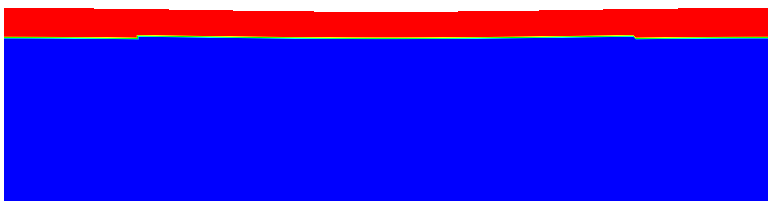
\includegraphics[width=0.95\textwidth]{cookbooks/benchmarks/crameri_et_al/doc/initial_topography.png}
  \end{center}
  \caption{\it Setup for the topography relaxation benchmark. The box is $2800$ km wide and $700$ km high, with
    a $100$ km lid on top. The lid has a viscosity of $10^{23} \, {Pa\,s}$, while the mantle has a viscosity of $10^{21} \, {Pa\,s}$.  The sides are
    free slip, the bottom is no slip, and the top is a free surface.  Both the lid and the mantle have
    a density of $3300 \,{kg/m^3}$, and gravity is $10 \, {m/s^2}$. There is a $7 \, {km}$
    sinusoidal initial topography on the free surface.}
  \label{fig:crameri-benchmark-initial-topography}
\end{figure}

The complete parameter file for this benchmark can be found in
\url{benchmarks/crameri_et_al/case_1/crameri_benchmark_1.prm},
the  most relevant parts of which are excerpted here:
\lstinputlisting[language=prmfile]{cookbooks/benchmarks/crameri_et_al/doc/crameri_benchmark_1.prm.out}
In particular, this benchmark uses a custom geometry model to set the initial geometry.
This geometry model, called ``\texttt{ReboundBox}'', is based on the \texttt{Box} geometry model.
It generates a domain in using the same parameters as \texttt{Box}, but then displaces all
the nodes vertically with a sinusoidal perturbation, where the magnitude and order of that
perturbation are specified in the \texttt{ReboundBox} subsection.


The characteristic timescales of topography relaxation are significantly smaller than those of
mantle convection. Taking timesteps larger than this relaxation timescale tends to cause sloshing
instabilities, which are described further in Section~\ref{sec:freesurface}. Some sort of stabilization
is required to take large timesteps. In this benchmark, however, we are interested in the relaxation
timescale, so we are free to take very small timesteps (in this case, 0.01 times the CFL
number).  As can be seen in Figure~\ref{fig:crameri-benchmark-relaxation-topography}, the results of all the
codes which are included in this comparison are basically indistinguishable.

\begin{figure}
  \begin{center}
    \includesvg[width=0.95\textwidth]{cookbooks/benchmarks/crameri_et_al/doc/crameri_1_comparison.svg}
  \end{center}
  \caption{\it Results for the topography relaxation benchmark, showing maximum topography
   versus time. Over about $100$ ka the topography completely disappears. The results of four
   free surface codes, as well as the semi-analytic solution, are nearly identical.}
  \label{fig:crameri-benchmark-relaxation-topography}
\end{figure}

\paragraph{Case 2: Dynamic topography.}
\label{sec:benchmark-crameri-case-2}

Case two is more complicated. Unlike the case one, it occurs over mantle convection
timescales.  In this benchmark there is the same high viscosity lid over a lower
viscosity mantle. However, now there is a blob of buoyant material rising in the
center of the domain, causing dynamic topography at the surface. The details for the setup
are in the caption of Figure~\ref{fig:crameri-benchmark-rising-blob}.

\begin{figure}
  \begin{center}
    
\includegraphics[width=0.95\textwidth]{cookbooks/benchmarks/crameri_et_al/doc/rising_blob.png}
  \end{center}
  \caption{\it Setup for the dynamic topography benchmark. Again, the domain is $2800$ km
  wide and $700$ km high.  A $100$ km thick lid with viscosity $10^{23}$ overlies a mantle
  with viscosity $10^{21}$.  Both the lid and the mantle have a density of $3300\,kg/m^3$.
  A blob with diameter $100$ km lies $300$ km from the bottom of the domain.  The blob has
  a density of $3200 kg/m^3$ and a viscosity of $10^{20}$ Pa s.}
  \label{fig:crameri-benchmark-rising-blob}
\end{figure}

Case two requires higher resolution and longer time integrations than case one. The benchmark
is over 20 million years and builds dynamic topography of $\sim 800$ meters.

\begin{figure}
  \begin{center}
    \includesvg[width=0.95\textwidth]{cookbooks/benchmarks/crameri_et_al/doc/crameri_2_comparison.svg}
  \end{center}
  \caption{\it Evolution of topography for the dynamic topography benchmark. The maximum topography
   is shown as a function of time, for \aspect{} as well as for several other codes participating in
   the benchmark. This benchmark shows considerably more scatter between the codes.}
  \label{fig:crameri-2-comparison}
\end{figure}

Again, we excerpt the most relevant parts of the parameter file for this benchmark, with the
full thing available in \url{benchmarks/crameri_et_al/case_2/crameri_benchmark_2.prm}.
Here we use the ``Multicomponent'' material model, which allows us to easily set up a number
of compositional fields with different material properties. The first compositional field
corresponds to background mantle, the second corresponds to the rising blob, and the third
corresponds to the viscous lid.


Furthermore, the results of this benchmark are sensitive to the mesh refinement and timestepping
parameters. Here we have nine refinement levels, and refine according to density and the
compositional fields.

\lstinputlisting[language=prmfile]{cookbooks/benchmarks/crameri_et_al/doc/crameri_benchmark_2.prm.out}

Unlike the first benchmark, for case two there is no (semi) analytical solution to compare against.
Furthermore, the time integration for this benchmark is much longer, allowing for errors to
accumulate. As such, there is considerably more scatter between the participating codes.  \aspect{}
does, however, fall within the range of the other results, and the curve is somewhat less wiggly.
The results for maximum topography versus time are shown in~\ref{fig:crameri-2-comparison}

The precise values for topography at a given time are quite dependent on the resolution and
timestepping parameters. Following \cite{CSG12} we investigate the convergence of the maximum
topography at 3 Ma as a function of CFL number and mesh resolution.  The results are shown in
figure~\ref{fig:crameri-benchmark-convergence}.

\begin{figure}
  \begin{center}
    \includesvg[width=1.0\textwidth]{cookbooks/benchmarks/crameri_et_al/doc/crameri_2_convergence.svg}
  \end{center}
  \caption{\it Convergence for case two.  Left: Logarithm of the error with decreasing CFL number.
As the CFL number decreases, the error gets smaller. However, once it reaches a value of $\sim0.1$, there
stops being much improvement in accuracy. Right: Logarithm of the error with increasing maximum mesh
resolution. As the resolution increases, so does the accuracy.}
  \label{fig:crameri-benchmark-convergence}
\end{figure}

We find that at 3 Ma \aspect{}  converges to a maximum topography of $\sim$396 meters.
This is slightly different from what MILAMIN\_VEP reported as its convergent value in \cite{CSG12},
but still well within the range of variation of the codes. Additionally, we note that \aspect{}
is able to achieve good results with relatively less mesh resolution due to the ability
to adaptively refine in the regions of interest (namely, the blob and the high viscosity lid).

Accuracy improves roughly linearly with decreasing CFL number, though stops improving at CFL $\sim 0.1$.
Accuracy also improves with increasing mesh resolution, though its convergence order does not seem
to be excellent.  It is possible that other mesh refinement parameters than we tried in this benchmark
could improve the convergence. The primary challenge in accuracy is limiting numerical diffusion
of the rising blob. If the blob becomes too diffuse, its ability to lift topography is diminished.
It would be instructive to compare the results of this benchmark using particles with the
results using compositional fields.
